\documentclass[12pt,a4paper]{yaac-luatex}

% Configurar geometry después de cargar la clase
\usepackage[margin=2.5cm,headheight=22pt]{geometry}

% ============= PAQUETES ADICIONALES =============
\usepackage{graphicx}
\usepackage{xcolor}
\usepackage{colortbl}  % Para \rowcolor en tablas
\usepackage{tikz}
\usetikzlibrary{shapes.geometric, positioning, shadows, arrows.meta}
\usepackage{fancyhdr}
\usepackage{tcolorbox}
\tcbuselibrary{skins,breakable}
\usepackage{enumitem}
\usepackage{multicol}
\usepackage{hyperref}
\usepackage{booktabs}
\usepackage{tabularx}
\usepackage{background}
\usepackage{eso-pic}
\usepackage{transparent}
\usepackage{tasks}

% Comandos para simular iconos fontawesome
\newcommand{\faInfoCircle}{\textbullet}
\newcommand{\faCalendar}{[Cal]}
\newcommand{\faClock}{[Time]}
\newcommand{\faBookReader}{[Read]}
\newcommand{\faUserGraduate}{[Grad]}
\newcommand{\faUsers}{[Group]}
\newcommand{\faChalkboardTeacher}{[Prof]}
\newcommand{\faUser}{[User]}
\newcommand{\faEnvelope}{[Email]}
\newcommand{\faGlobe}{[Web]}
\newcommand{\faRobot}{[AI]}
\newcommand{\faBookOpen}{[Book]}
\newcommand{\faFileAlt}{[File]}
\newcommand{\faStream}{[\textasciitilde]}
\newcommand{\faChartBar}{[Chart]}
\newcommand{\faBook}{[Bk]}

% ============= COLORES INSTITUCIONALES =============
\definecolor{maincolor}{RGB}{0, 102, 204}      % Azul UNSCH
\definecolor{accentcolor}{RGB}{255, 153, 0}    % Naranja acento
\definecolor{darkgray}{RGB}{51, 51, 51}
\definecolor{lightgray}{RGB}{240, 240, 240}
\definecolor{mediumgray}{RGB}{180, 180, 180}
\definecolor{curso1color}{RGB}{46, 125, 50}    % Verde para Curso IA
\definecolor{curso2color}{RGB}{211, 47, 47}    % Rojo para Curso APA/Vancouver
\definecolor{curso3color}{RGB}{123, 31, 162}   % Morado para Curso Monografías

% ============= CONFIGURACIÓN DE ENLACES =============
\hypersetup{
	colorlinks=true,
	linkcolor=maincolor,
	urlcolor=maincolor,
	citecolor=maincolor,
	pdfauthor={Edison Achalma, B.S.},
	pdftitle={Programa Integrado: IA + APA/Vancouver + Monografías},
	pdfsubject={Tres Cursos para Investigación Académica Universitaria}
}

% ============= MARCA DE AGUA =============
\backgroundsetup{
	scale=1,
	angle=0,
	opacity=0.05,
	contents={
		\begin{tikzpicture}[remember picture,overlay]
			\node[anchor=center] at (current page.center) {
				
\includegraphics[width=12cm]{cau-logo}
			};
		\end{tikzpicture}
	}
}

% ============= ENCABEZADO Y PIE DE PÁGINA =============
% Redefinir el estilo 'plain' para que sea IGUAL al estilo 'fancy' (incluye tu header y regla)
\fancypagestyle{plain}{%
	\fancyhf{}  % limpia todo primero (por seguridad)
	\fancyhead[L]{\small\color{maincolor}\textbf{CAU - UNSCH | Programa Investigación 2026}}
	\fancyhead[R]{\small\color{darkgray}Semestre 2026-I}
	\fancyfoot[C]{\small\color{mediumgray}\thepage}
	\renewcommand{\headrulewidth}{0.5pt}
	\renewcommand{\headrule}{%
		\hbox to\headwidth{\color{maincolor}\leaders\hrule height \headrulewidth\hfill}%
	}
	% Si también quieres conservar la línea del footer (opcional)
	\renewcommand{\footrulewidth}{0.4pt}  % o 0pt si no quieres línea abajo
}

% ============= COMANDOS PERSONALIZADOS =============
\newcommand{\cursotitulo}[2]{
	\vspace{0.5cm}
	\begin{tcolorbox}[
		enhanced,
		colback=#1,
		colframe=#1,
		arc=5pt,
		boxrule=0pt,
		left=12pt,
		right=12pt,
		top=10pt,
		bottom=10pt
		]
		{\color{white}\Large\bfseries #2}
	\end{tcolorbox}
}

\newcommand{\secciontitulo}[1]{
	\vspace{0.5cm}
	\begin{tcolorbox}[
		enhanced,
		colback=maincolor,
		colframe=maincolor,
		arc=3pt,
		boxrule=0pt,
		left=8pt,
		right=8pt,
		top=6pt,
		bottom=6pt
		]
		{\color{white}\large\bfseries #1}
	\end{tcolorbox}
}

\newcommand{\subsecciontitulo}[1]{
	{\color{maincolor}\large\bfseries #1}
}

\newcommand{\icontext}[2]{
	\mbox{%
		\textcolor{maincolor}{#1}\hspace{0.3em}%
		{#2}%
	}%
}

\newcommand{\destacado}[1]{
	\colorbox{lightgray}{\textbf{#1}}
}

% ============= INICIO DEL DOCUMENTO =============
\begin{document}
	
	% ============= PORTADA =============
	\begin{titlepage}
		\centering
		
		% Logo institucional
		\vspace*{1cm}
		
\includegraphics[width=5cm]{cau-logo}
		
		\vspace{1.5cm}
		
		% Título principal
		{\Huge\bfseries\color{maincolor}
			Programa Integrado de\\
			Investigación Académica\\[0.3cm]
		}
		
		\vspace{0.5cm}
		
		{\Large\color{accentcolor}\bfseries
			Inteligencia Artificial + APA/Vancouver + Monografías
		}
		
		\vspace{1cm}
		
		% Información del programa
		\begin{tcolorbox}[
			enhanced,
			colback=white,
			colframe=maincolor,
			arc=3pt,
			boxrule=2pt,
			left=15pt,
			right=15pt,
			top=12pt,
			bottom=12pt,
			width=0.9\textwidth
			]
			\centering
			{\Large\bfseries Tres Cursos Complementarios}\\[0.5cm]
			
			\begin{minipage}{0.45\textwidth}
				\centering
				{\color{curso1color}\Large\faRobot}\\[0.2cm]
				{\large\bfseries Curso 1}\\
				Inteligencia Artificial\\
				para Universitarios\\[0.3cm]
				{\small 8 sesiones | 16 horas}
			\end{minipage}
			\hfill
			\begin{minipage}{0.45\textwidth}
				\centering
				{\color{curso2color}\Large\faBookOpen}\\[0.2cm]
				{\large\bfseries Curso 2}\\
				Sistemas APA 7ª\\
				y Vancouver\\[0.3cm]
				{\small 8 sesiones | 16 horas}
			\end{minipage}
			
			\vspace{0.5cm}
			
			\begin{minipage}{0.45\textwidth}
				\centering
				{\color{curso3color}\Large\faFileAlt}\\[0.2cm]
				{\large\bfseries Curso 3}\\
				Elaboración de\\
				Monografías\\[0.3cm]
				{\small 8 sesiones | 16 horas}
			\end{minipage}
			
		\end{tcolorbox}
		
		\vspace{1cm}
		
		% Datos básicos
		\begin{minipage}{0.45\textwidth}
			\begin{tcolorbox}[
				enhanced,
				colback=lightgray,
				colframe=darkgray,
				arc=3pt,
				boxrule=1pt,
				left=10pt,
				right=10pt,
				top=8pt,
				bottom=8pt
				]
				\icontext{\faCalendar}{Duración: 12 semanas}\\[0.2cm]
				\icontext{\faClock}{Total: 48 horas}\\[0.2cm]
				\icontext{\faBookReader}{24 sesiones × 2 horas}
			\end{tcolorbox}
		\end{minipage}
		\hfill
		\begin{minipage}{0.45\textwidth}
			\begin{tcolorbox}[
				enhanced,
				colback=lightgray,
				colframe=darkgray,
				arc=3pt,
				boxrule=1pt,
				left=10pt,
				right=10pt,
				top=8pt,
				bottom=8pt
				]
				\icontext{\faUserGraduate}{Nivel: Cachimbos}\\[0.2cm]
				\icontext{\faUsers}{Todas las disciplinas}\\[0.2cm]
				\icontext{\faChalkboardTeacher}{Modalidad: Presencial}
			\end{tcolorbox}
		\end{minipage}
		
		\vfill
		
		% Información del docente
		\begin{tcolorbox}[
			enhanced,
			colback=white,
			colframe=darkgray,
			arc=3pt,
			boxrule=1pt,
			left=12pt,
			right=12pt,
			top=10pt,
			bottom=10pt
			]
			{\color{maincolor}\Large\bfseries\faUser \hspace{0.3em} Docente}\\[0.3cm]
			{\large\bfseries Edison Achalma, B.S.}\\[0.1cm]
			{\normalsize Economista | Data Science e IA | Software Libre}\\[0.2cm]
			\icontext{\faEnvelope}{elmer.achalma.09@unsch.edu.pe}\\[0.1cm]
			\icontext{\faGlobe}{\href{https://github.com/achalmed}{github.com/achalmed}}\\[0.1cm]
			\icontext{\faClock}{Consultas: Miércoles 15:00-17:00 hrs}
		\end{tcolorbox}
		
		\vspace{0.5cm}
		{\color{mediumgray}\small Centro de Actualización Universitaria (CAU)}\\
		{\color{mediumgray}\small Universidad Nacional de San Cristóbal de Huamanga}\\
		{\color{mediumgray}\small Ayacucho, Perú | 2026-I}
		
	\end{titlepage}
	
	% ============= CONTENIDO DEL PROGRAMA =============
	\newpage
	
	% ============= I. PRESENTACIÓN GENERAL =============
	\secciontitulo{\faInfoCircle \hspace{0.3em} I. PRESENTACIÓN GENERAL DEL PROGRAMA}
	
	\subsection*{Contexto y Justificación}
	
	En la era de la información digital (2026), los universitarios de \textbf{todas las disciplinas}---Medicina, Economía, Ingenierías, Matemáticas, Humanidades, Ciencias Sociales---enfrentan tres desafíos críticos para su formación académica:
	
	\begin{enumerate}[leftmargin=*, itemsep=0.3cm]
		\item \textbf{Inteligencia Artificial}: Necesitan dominar herramientas de IA (ChatGPT, Gemini, Grok) y técnicas de prompt engineering para investigación, análisis de datos y redacción académica de forma ética y responsable.
		
		\item \textbf{Sistemas de Citación}: Deben aplicar correctamente sistemas profesionales de citación (APA 7ª edición, Vancouver) usando gestores bibliográficos modernos (Zotero) para evitar plagio y mantener integridad académica.
		
		\item \textbf{Escritura Académica}: Requieren competencias para elaborar monografías, papers y trabajos de investigación con metodología rigurosa, desde la delimitación del tema hasta la defensa final.
	\end{enumerate}
	
	Este programa integra estos tres componentes en un \textbf{ecosistema coherente de aprendizaje}, donde cada curso se complementa con los otros para desarrollar competencias investigativas integrales.
	
	\subsection*{Enfoque Pedagógico}
	
	El programa adopta una metodología \textbf{learning-by-doing} con énfasis en:
	
	\begin{itemize}[leftmargin=*, itemsep=0.2cm]
		\item \textbf{Práctica intensiva}: 60\% prácticas hands-on, 40\% teoría
		\item \textbf{Trabajo interdisciplinario}: Grupos con estudiantes de diferentes carreras
		\item \textbf{Software libre}: Todas las herramientas son gratuitas y de código abierto
		\item \textbf{Evaluación formativa}: Feedback cualitativo continuo sin calificaciones numéricas
		\item \textbf{Proyecto integrador}: Monografía final que integra IA, citación profesional y escritura académica
	\end{itemize}
	
	\subsection*{Objetivos Generales del Programa}
	
	Al finalizar el programa completo (48 horas), los estudiantes serán capaces de:
	
	\begin{enumerate}[leftmargin=*, itemsep=0.2cm]
		\item \textbf{Dominar} técnicas avanzadas de prompt engineering con 16 frameworks para investigación académica
		\item \textbf{Gestionar} referencias bibliográficas con Zotero y aplicar sistemas APA 7ª/Vancouver de forma automática
		\item \textbf{Organizar} conocimiento con Obsidian (notas Markdown, mapas conceptuales, backlinks)
		\item \textbf{Elaborar} monografías completas integrando IA, fuentes verificadas y citación ética
		\item \textbf{Evaluar críticamente} outputs de IA, detectar sesgos y aplicar principios éticos en investigación
		\item \textbf{Utilizar} herramientas de investigación avanzadas: Google NotebookLM, Scite, Elicit, Connected Papers
	\end{enumerate}
	
	\subsection*{Competencias Transversales}
	
	\begin{tcolorbox}[
		enhanced,
		colback=lightgray,
		colframe=maincolor,
		arc=3pt,
		boxrule=1pt,
		breakable
		]
		\begin{itemize}[leftmargin=*, itemsep=0.2cm]
			\item \textbf{Pensamiento crítico}: Analizar fuentes, evaluar calidad de información, detectar sesgos
			\item \textbf{Alfabetización digital}: Dominar ecosistema de herramientas para investigación moderna
			\item \textbf{Ética académica}: Comprender y aplicar principios de integridad, citación correcta, uso responsable de IA
			\item \textbf{Aprendizaje autónomo}: Gestionar conocimiento personal con sistemas como Zettelkasten
			\item \textbf{Comunicación académica}: Redactar textos claros, rigurosos y bien fundamentados
		\end{itemize}
	\end{tcolorbox}
	
	\subsection*{Requisitos y Recursos}
	
	\textbf{Requisitos previos:}
	\begin{itemize}[leftmargin=*, itemsep=0.1cm]
		\item Ninguno (curso diseñado para cachimbos de cualquier carrera)
		\item Curiosidad intelectual y disposición para aprender
		\item Laptop/PC con conexión a internet
	\end{itemize}
	
	\textbf{Software requerido (todo gratuito):}
	\begin{multicols}{2}
		\begin{itemize}[leftmargin=*, itemsep=0.1cm]
			\item ChatGPT / Grok / Gemini
			\item \textbf{Zotero + plugins}
			\item \textbf{Obsidian}
			\item Google NotebookLM
			\item VS Code
			\item Google Colab
			\item Word / LibreOffice
			\item Canva (versión gratuita)
		\end{itemize}
	\end{multicols}
	
	\newpage
	
	% ============= II. ESTRUCTURA DEL PROGRAMA =============
	\secciontitulo{\faStream \hspace{0.3em} II. ESTRUCTURA DEL PROGRAMA}
	
	El programa está organizado en \textbf{tres cursos complementarios} que se imparten de forma secuencial, con un total de \textbf{24 sesiones de 2 horas} cada una (48 horas totales):
	
	\vspace{0.5cm}
	
	\begin{center}
		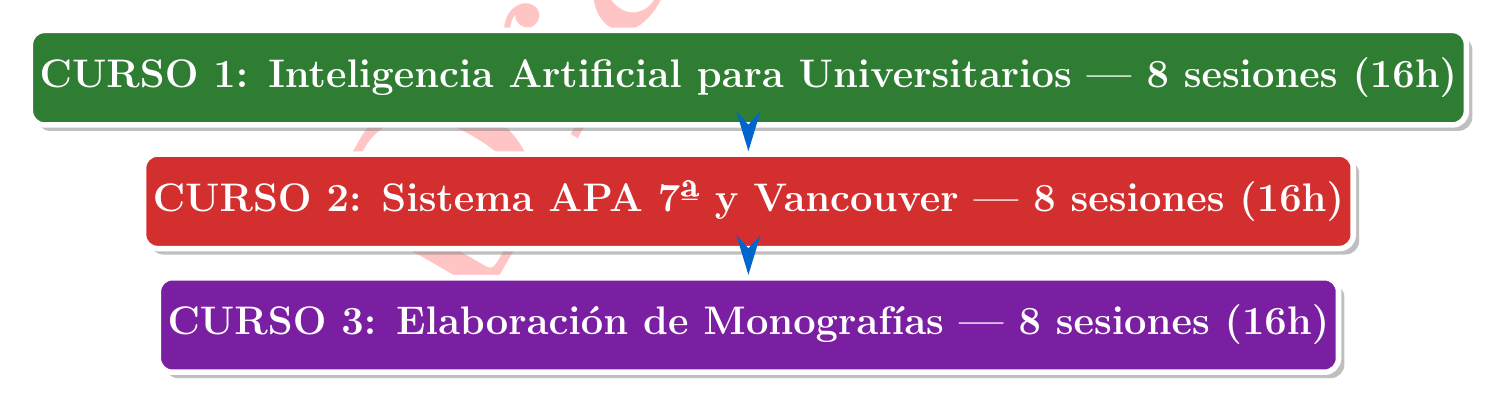
\begin{tikzpicture}[
			node distance=0.3cm,
			curso/.style={
				rectangle,
				rounded corners=5pt,
				minimum width=10cm,
				minimum height=1.2cm,
				text centered,
				draw=white,
				line width=2pt,
				font=\bfseries,
				drop shadow
			}
			]
			
			\node[curso, fill=curso1color, text=white] (c1) 
			{\Large CURSO 1: Inteligencia Artificial para Universitarios | 8 sesiones (16h)};
			
			\node[curso, fill=curso2color, text=white, below=of c1] (c2)
			{\Large CURSO 2: Sistema APA 7ª y Vancouver | 8 sesiones (16h)};
			
			\node[curso, fill=curso3color, text=white, below=of c2] (c3)
			{\Large CURSO 3: Elaboración de Monografías | 8 sesiones (16h)};
			
			\draw[-{Stealth[length=5mm, width=3mm]}, line width=2pt, maincolor] 
			(c1.south) -- (c2.north);
			
			\draw[-{Stealth[length=5mm, width=3mm]}, line width=2pt, maincolor] 
			(c2.south) -- (c3.north);
			
		\end{tikzpicture}
	\end{center}
	
	\vspace{0.5cm}
	
	\subsection*{Cronograma General}
	
	\begin{table}[h]
		\centering
		\begin{tabular}{|l|c|c|c|}
			\hline
			\rowcolor{maincolor}
			\textcolor{white}{\textbf{Curso}} & \textcolor{white}{\textbf{Semanas}} & \textcolor{white}{\textbf{Sesiones}} & \textcolor{white}{\textbf{Horas}} \\
			\hline
			Curso 1: Inteligencia Artificial & 1-4 & 8 sesiones & 16 horas \\
			\hline
			Curso 2: APA 7ª y Vancouver + Zotero & 5-8 & 8 sesiones & 16 horas \\
			\hline
			Curso 3: Elaboración de Monografías & 9-12 & 8 sesiones & 16 horas \\
			\hline
			\rowcolor{lightgray}
			\textbf{TOTAL} & \textbf{12 semanas} & \textbf{24 sesiones} & \textbf{48 horas} \\
			\hline
		\end{tabular}
	\end{table}
	
	\subsection*{Modalidad de Evaluación}
	
	El programa utiliza un sistema de \textbf{evaluación formativa continua} sin calificaciones numéricas:
	
	\begin{itemize}[leftmargin=*, itemsep=0.2cm]
		\item \textbf{Curso 1}: Portafolio de prompts (30\%) + Ejercicio integrador de IA (20\%)
		\item \textbf{Curso 2}: Biblioteca Zotero con 30+ fuentes (30\%) + Documento con citación APA/Vancouver (20\%)
		\item \textbf{Curso 3}: Monografía completa (60\%) + Presentación oral (20\%) + Reflexión ética (20\%)
	\end{itemize}
	
	\textbf{Requisito mínimo de asistencia:} 80\% en cada curso
	
	\newpage
	
	% ============================================================
	% CURSO 1: INTELIGENCIA ARTIFICIAL PARA UNIVERSITARIOS
	% ============================================================
	
	\cursotitulo{curso1color}{\faRobot \hspace{0.5em} CURSO 1: INTELIGENCIA ARTIFICIAL PARA UNIVERSITARIOS}
	
	\vspace{0.3cm}
	
	\begin{tcolorbox}[
		enhanced,
		colback=white,
		colframe=curso1color,
		arc=3pt,
		boxrule=2pt,
		breakable
		]
		\textbf{Duración:} | 8 sesiones de 2 horas | Total: 16 horas\\[0.2cm]
		\textbf{Objetivo:} Desarrollar competencias en el uso ético y efectivo de herramientas de Inteligencia Artificial para investigación, análisis y redacción académica mediante técnicas avanzadas de prompt engineering.
	\end{tcolorbox}
	
	\subsection*{Temario}
	
	% ===== SESIÓN 1-2: Introducción a IA =====
	\begin{tcolorbox}[
		enhanced,
		colback=white,
		colframe=curso1color,
		arc=3pt,
		boxrule=1.5pt,
		left=10pt,
		right=10pt,
		top=8pt,
		bottom=8pt,
		breakable
		]
		\subsecciontitulo{Sesiones 1-2: Introducción a la IA y Primeros Pasos (4 horas)}
		
		\textbf{Contenidos:}
		\begin{itemize}[leftmargin=*, itemsep=0.1cm]
			\item ¿Qué es la IA? Mitos vs. Realidad en 2026
			\item Historia breve: De ELIZA a GPT-4 y modelos multimodales
			\item Aplicaciones por disciplina:
			\begin{itemize}
				\item Medicina: Diagnóstico asistido, análisis de literatura médica
				\item Economía: Análisis predictivo, interpretación de datos
				\item Ingeniería: Simulación, optimización de diseños
				\item Humanidades: Análisis textual, traducción, investigación histórica
			\end{itemize}
			\item Modelos disponibles: ChatGPT, Grok, Gemini, Claude, Llama 3.3
			\item Principios éticos fundamentales:
			\begin{itemize}
				\item Transparencia en el uso de IA
				\item Privacidad y protección de datos
				\item Detección y mitigación de sesgos
				\item Responsabilidad académica
			\end{itemize}
			\item Primera interacción: Anatomía de un prompt simple
		\end{itemize}
		
		\textbf{Prácticas:}
		\begin{itemize}[leftmargin=*, itemsep=0.1cm]
			\item Lab: Crear cuentas en ChatGPT/Grok/Gemini
			\item Ejercicio 1: Ejecutar 5 prompts básicos para tu disciplina
			\item Ejercicio 2: Brainstorming de ideas para proyecto final usando IA
			\item Tarea: Reflexión escrita (1 página): "¿Cómo puede la IA transformar mi carrera?"
		\end{itemize}
	\end{tcolorbox}
	
	\vspace{0.3cm}
	
	% ===== SESIÓN 3-4: Prompt Engineering =====
	\begin{tcolorbox}[
		enhanced,
		colback=white,
		colframe=curso1color,
		arc=3pt,
		boxrule=1.5pt,
		left=10pt,
		right=10pt,
		top=8pt,
		bottom=8pt,
		breakable
		]

		\subsecciontitulo{Sesiones 3-4: Prompt Engineering - 16 Frameworks (4 horas)}
	
	\textbf{Contenidos:}
	\begin{itemize}[leftmargin=*, itemsep=0.1cm]
		\item Anatomía de un prompt efectivo: Rol - Tarea - Contexto - Formato - Restricciones
		\item \textbf{16 Frameworks esenciales:}
		\begin{multicols}{2}
			\begin{enumerate}[leftmargin=*, itemsep=0.05cm]
				\item \textbf{RTF} (Role-Task-Format)
				\item \textbf{APE} (Action-Purpose-Expectation)
				\item \textbf{CHAT} (Context-History-Action-Task)
				\item \textbf{ROSES} (Role-Objective-Scenario-Expected-Solution)
				\item \textbf{LangGPT} (Language-Goal-Process-Tone)
				\item \textbf{SCOPE} (Situation-Complication-Objective-Plan-Evaluation)
				\item \textbf{TRACE} (Task-Request-Action-Context-Example)
				\item \textbf{SPAR} (Situation-Problem-Action-Result)
				\item \textbf{CARE} (Context-Action-Result-Example)
				\item \textbf{COAST} (Context-Objective-Actions-Scenario-Task)
				\item \textbf{RACE} (Role-Action-Context-Expectation)
				\item \textbf{RISE} (Role-Input-Steps-Expectation)
				\item \textbf{SAGE} (Situation-Action-Goal-Expectation)
				\item \textbf{TAG} (Task-Action-Goal)
				\item \textbf{CRISPE} (Capacity-Role-Insight-Statement-Personality-Experiment)
				\item \textbf{SMART} (Specific-Measurable-Achievable-Relevant-Time-bound)
			\end{enumerate}
		\end{multicols}
		\item Cuándo usar cada framework según el tipo de tarea
		\item Ejemplos aplicados a cada disciplina
	\end{itemize}
	
	\textbf{Prácticas:}
	\begin{itemize}[leftmargin=*, itemsep=0.1cm]
		\item Lab: Diseñar 16 prompts (uno por cada framework) para temas de tu carrera
		\item Ejercicio comparativo: Mismo problema, 5 frameworks diferentes
		\item Workshop grupal: Crear biblioteca de prompts por disciplina
		\item Tarea: Portafolio de 20 prompts personalizados
	\end{itemize}
	\end{tcolorbox}
	
	\vspace{0.3cm}
	
	% ===== SESIÓN 5-6: Gestión de Conocimiento =====
	\begin{tcolorbox}[
		enhanced,
		colback=white,
		colframe=curso1color,
		arc=3pt,
		boxrule=1.5pt,
		left=10pt,
		right=10pt,
		top=8pt,
		bottom=8pt,
		breakable
		]
		\subsecciontitulo{Sesiones 5-6: Obsidian y Markdown para Gestión de Conocimiento (4 horas)}
		
		\textbf{Contenidos:}
		\begin{itemize}[leftmargin=*, itemsep=0.1cm]
			\item ¿Por qué Obsidian? Filosofía del "Second Brain"
			\item Instalación y configuración inicial
			\item \textbf{Markdown esencial}:
			\begin{itemize}
				\item Headers, énfasis (negrita, cursiva)
				\item Listas ordenadas y no ordenadas
				\item Enlaces externos e imágenes
				\item Bloques de código
				\item Tablas y checkboxes
			\end{itemize}
			\item \textbf{Sistema Zettelkasten}:
			\begin{itemize}
				\item Concepto de notas atómicas
				\item Enlaces bidireccionales [[nombre-nota]]
				\item Tags y carpetas
				\item Grafo de conocimiento
			\end{itemize}
			\item Flujo de trabajo: Capturar → Procesar → Conectar → Crear
			\item Plugins esenciales: Dataview, Templater, Calendar
		\end{itemize}
		
		\textbf{Prácticas:}
		\begin{itemize}[leftmargin=*, itemsep=0.1cm]
			\item Lab: Instalar Obsidian y crear primer vault
			\item Ejercicio 1: Crear 20 notas atómicas interconectadas sobre un tema de tu carrera
			\item Ejercicio 2: Usar IA para generar contenido y organizarlo en Obsidian
			\item Tarea: Vault personal con 50+ notas para tu proyecto final
		\end{itemize}
	\end{tcolorbox}
	
	\vspace{0.3cm}
	
	% ===== SESIÓN 7-8: Herramientas Avanzadas =====
	\begin{tcolorbox}[
		enhanced,
		colback=white,
		colframe=curso1color,
		arc=3pt,
		boxrule=1.5pt,
		left=10pt,
		right=10pt,
		top=8pt,
		bottom=8pt,
		breakable
		]
		\subsecciontitulo{Sesiones 7-8: Herramientas Avanzadas de Investigación con IA (4 horas)}
		
		\textbf{Contenidos:}
		\begin{itemize}[leftmargin=*, itemsep=0.1cm]
			\item \textbf{Google NotebookLM:}
			\begin{itemize}
				\item Subir PDFs y crear notas automáticas
				\item Generar podcasts de audio de tus fuentes
				\item Integración con Obsidian
				\item Hacer preguntas específicas a corpus de documentos
			\end{itemize}
			\item \textbf{Plataformas de investigación académica:}
			\begin{itemize}
				\item \textbf{Scite}: Verificar cómo artículos citan a otros (supporting/contrasting)
				\item \textbf{Elicit}: Buscar papers con IA, extraer insights
				\item \textbf{Scispace}: Copilot para papers, explicaciones contextuales
				\item \textbf{Connected Papers}: Grafo visual de literatura relacionada
			\end{itemize}
			\item \textbf{OCR con IA:}
			\begin{itemize}
				\item Google Drive OCR para digitalizar documentos escaneados
				\item Adobe Acrobat OCR
				\item Tesseract + Python para batch processing
			\end{itemize}
			\item \textbf{Transcripción automática:}
			\begin{itemize}
				\item Google Colab + Whisper para transcribir entrevistas/clases
				\item Otter.ai, Trint
			\end{itemize}
			\item Flujo integrado: Buscar (Elicit) → Verificar (Scite) → Mapear (Connected Papers) → Resumir (NotebookLM) → Organizar (Obsidian)
		\end{itemize}
		
		\textbf{Prácticas:}
		\begin{itemize}[leftmargin=*, itemsep=0.1cm]
			\item Lab 1: Usar NotebookLM para generar resumen + podcast de 5 PDFs
			\item Lab 2: Explorar red de papers con Connected Papers
			\item Lab 3: Transcribir audio de 10 minutos con Whisper
			\item Lab 4: Digitalizar documento antiguo con OCR
			\item Tarea: Investigación preliminar para monografía final usando estas 4 herramientas
		\end{itemize}
	\end{tcolorbox}
	
	\vspace{0.5cm}
	
	\subsection*{Evaluación del Curso 1}
	
	\begin{itemize}[leftmargin=*, itemsep=0.2cm]
		\item \textbf{Portafolio de Prompts} (50\%): Colección de 40 prompts efectivos usando los 16 frameworks, aplicados a problemas reales de tu disciplina
		\item \textbf{Vault de Obsidian} (30\%): Bóveda con 50+ notas atómicas interconectadas, incluyendo contenido generado con IA
		\item \textbf{Ejercicio Integrador} (20\%): Informe de investigación preliminar (5-7 páginas) usando NotebookLM, Scite, Elicit, Connected Papers
	\end{itemize}
	
	\newpage
	
	% ============================================================
	% CURSO 2: SISTEMAS APA 7ª Y VANCOUVER + ZOTERO
	% ============================================================
	
	\cursotitulo{curso2color}{\faBookOpen \hspace{0.5em} CURSO 2: SISTEMAS APA 7ª Y VANCOUVER}
	
	\vspace{0.3cm}
	
	\begin{tcolorbox}[
		enhanced,
		colback=white,
		colframe=curso2color,
		arc=3pt,
		boxrule=2pt,
		breakable
		]
		\textbf{Duración:}  | 8 sesiones de 2 horas | Total: 16 horas\\[0.2cm]
		\textbf{Objetivo:} Dominar los sistemas de citación profesional APA 7ª edición y Vancouver mediante el uso avanzado del gestor bibliográfico Zotero, aplicando principios de software libre y gestión eficiente de referencias.
	\end{tcolorbox}
	
	\subsection*{Temario}
	
	% ===== SESIÓN 1-2: Zotero Básico =====
	\begin{tcolorbox}[
		enhanced,
		colback=white,
		colframe=curso2color,
		arc=3pt,
		boxrule=1.5pt,
		left=10pt,
		right=10pt,
		top=8pt,
		bottom=8pt,
		breakable
		]
		\subsecciontitulo{Sesiones 1-2: Instalación y Configuración de Zotero (4 horas)}
		
		\textbf{Contenidos:}
		\begin{itemize}[leftmargin=*, itemsep=0.1cm]
			\item \textbf{Filosofía del software libre aplicado a investigación}
			\begin{itemize}
				\item ¿Por qué Zotero vs. Mendeley/EndNote?
				\item Principios del software libre: Control, privacidad, comunidad
				\item Ecosistema abierto: Plugins, integraciones, personalización
			\end{itemize}
			\item \textbf{Instalación y configuración inicial}
			\begin{itemize}
				\item Descargar e instalar Zotero Desktop (Windows/Mac/Linux)
				\item Crear cuenta Zotero.org (almacenamiento gratuito 300 MB)
				\item Instalar Zotero Connector (Chrome/Firefox/Edge)
				\item Configurar sincronización en la nube
			\end{itemize}
			\item \textbf{Conceptos básicos}
			\begin{itemize}
				\item Biblioteca personal vs. Grupos
				\item Colecciones y subcolecciones (estructura de carpetas)
				\item Items: Artículo, libro, tesis, página web, etc.
				\item Metadatos: Autor, título, año, DOI, URL, etc.
				\item Archivos adjuntos (PDFs, imágenes)
			\end{itemize}
			\item \textbf{Primeras capturas}
			\begin{itemize}
				\item Añadir referencias desde Google Scholar
				\item Añadir desde PubMed, SciELO, JSTOR
				\item Añadir manualmente un libro
			\end{itemize}
		\end{itemize}
		
		\textbf{Prácticas:}
		\begin{itemize}[leftmargin=*, itemsep=0.1cm]
			\item Lab 1: Instalar Zotero + Connector, configurar cuenta
			\item Lab 2: Crear 3 colecciones para diferentes temas
			\item Lab 3: Importar 20 fuentes desde Google Scholar y bases de datos
			\item Tarea: Biblioteca básica con 30 referencias de tu disciplina
		\end{itemize}
	\end{tcolorbox}
	
	\vspace{0.3cm}
	
	% ===== SESIÓN 3-4: Zotero Intermedio =====
	\begin{tcolorbox}[
		enhanced,
		colback=white,
		colframe=curso2color,
		arc=3pt,
		boxrule=1.5pt,
		left=10pt,
		right=10pt,
		top=8pt,
		bottom=8pt,
		breakable
		]
		\subsecciontitulo{Sesiones 3-4: Gestión Avanzada de Zotero (4 horas)}
		
		\textbf{Contenidos:}
		\begin{itemize}[leftmargin=*, itemsep=0.1cm]
			\item \textbf{Métodos avanzados de captura}
			\begin{itemize}
				\item Añadir fuentes usando DOI o ISBN directamente
				\item Importar desde otros gestores (Mendeley, EndNote)
				\item Añadir PDFs y extraer metadatos automáticamente
				\item Guardar páginas web completas como fuentes citables
				\item Importar listas de resultados masivos (RIS, BibTeX)
			\end{itemize}
			\item \textbf{Organización eficiente}
			\begin{itemize}
				\item Crear colecciones y subcolecciones temáticas
				\item Sistema de etiquetas (tags): colores, jerarquías
				\item Búsquedas guardadas y colecciones inteligentes
				\item Cronografías: línea de tiempo visual
			\end{itemize}
			\item \textbf{Anotaciones y notas}
			\begin{itemize}
				\item Hacer anotaciones en PDFs dentro de Zotero
				\item Crear notas vinculadas a cada fuente
				\item Relaciones entre items: "Citado en", "Relacionado con"
			\end{itemize}
			\item \textbf{Gestión de archivos}
			\begin{itemize}
				\item Configurar almacén de datos
				\item Localizar archivos adjuntos
				\item Eliminar duplicados
				\item Renombrar PDFs automáticamente
			\end{itemize}
		\end{itemize}
		
		\textbf{Prácticas:}
		\begin{itemize}[leftmargin=*, itemsep=0.1cm]
			\item Lab 1: Importar 10 PDFs y extraer metadatos
			\item Lab 2: Crear sistema de etiquetas con 5 categorías
			\item Lab 3: Configurar colecciones inteligentes
			\item Tarea: Biblioteca organizada con 50+ fuentes, etiquetadas y anotadas
		\end{itemize}
	\end{tcolorbox}
	
	\vspace{0.3cm}
	
	% ===== SESIÓN 5-6: APA 7ª Edición =====
	\begin{tcolorbox}[
		enhanced,
		colback=white,
		colframe=curso2color,
		arc=3pt,
		boxrule=1.5pt,
		left=10pt,
		right=10pt,
		top=8pt,
		bottom=8pt,
		breakable
		]
		\subsecciontitulo{Sesiones 5-6: Sistema APA 7ª Edición (4 horas)}
		
		\textbf{Contenidos:}
		\begin{itemize}[leftmargin=*, itemsep=0.1cm]
			\item \textbf{Estructura general de trabajos APA}
			\begin{itemize}
				\item Portada: Título, autor, afiliación, nota del autor
				\item Resumen (Abstract)
				\item Cuerpo: Introducción, Método, Resultados, Discusión
				\item Referencias
				\item Apéndices, tablas y figuras
			\end{itemize}
			\item \textbf{Formato APA}
			\begin{itemize}
				\item Tamaño de página: Carta (8.5 × 11 pulgadas)
				\item Márgenes: 2.54 cm (1 pulgada)
				\item Fuentes: Times New Roman 12pt, Calibri 11pt, Arial 11pt
				\item Interlineado: Doble
				\item Alineación: Izquierda (no justificada)
				\item Encabezados: Número de página alineado a la derecha
				\item Niveles de títulos: 5 niveles jerárquicos
			\end{itemize}
			\item \textbf{Estilo APA: Comillas, cursivas, números, mayúsculas}
			\item \textbf{Citas textuales en APA}
			\begin{itemize}
				\item Cita narrativa vs. cita entre paréntesis
				\item Citas cortas (< 40 palabras): entre comillas
				\item Citas largas (≥ 40 palabras): bloque con sangría
				\item Un autor: (Sánchez, 2020) o Sánchez (2020)
				\item Dos autores: (Pérez \& Gómez, 2019)
				\item Tres o más autores: (López et al., 2021)
				\item Sin autor: (Título del artículo, 2022)
				\item Citas secundarias: (Original, año, como se citó en Secundaria, año)
			\end{itemize}
			\item \textbf{Referencias bibliográficas en APA}
			\begin{itemize}
				\item Estructura: Autor. (Año). \textit{Título}. Fuente. DOI/URL
				\item Libros: Apellido, I. (año). \textit{Título del libro}. Editorial.
				\item Artículos de revista: Apellido, I. (año). Título del artículo. \textit{Nombre de la Revista}, vol(núm), pp-pp. DOI
				\item Páginas web: Apellido, I. (año). Título de la página. Nombre del sitio. URL
				\item Casos especiales: Tesis, informes gubernamentales (ej. MINSA Perú), datasets, software, contenido de IA
			\end{itemize}
			\item \textbf{Configurar estilo APA en Zotero}
			\item \textbf{Insertar citas en Word con plugin Zotero}
		\end{itemize}
		
		\textbf{Prácticas:}
		\begin{itemize}[leftmargin=*, itemsep=0.1cm]
			\item Lab 1: Configurar Word con formato APA completo
			\item Lab 2: Insertar 15 citas de Zotero en documento Word (narrativas y paréntesis)
			\item Lab 3: Generar lista de referencias automática
			\item Lab 4: Citar contenido generado con ChatGPT según APA
			\item Tarea: Documento de 3 páginas con 10+ citas en APA perfectamente formateadas
		\end{itemize}
	\end{tcolorbox}
	
	\vspace{0.3cm}
	
	% ===== SESIÓN 7-8: Vancouver + Plugins =====
	\begin{tcolorbox}[
		enhanced,
		colback=white,
		colframe=curso2color,
		arc=3pt,
		boxrule=1.5pt,
		left=10pt,
		right=10pt,
		top=8pt,
		bottom=8pt,
		breakable
		]
		\subsecciontitulo{Sesiones 7-8: Sistema Vancouver + Plugins Avanzados de Zotero (4 horas)}
		
		\textbf{Contenidos:}
		\begin{itemize}[leftmargin=*, itemsep=0.1cm]
			\item \textbf{Sistema Vancouver}
			\begin{itemize}
				\item Uso en ciencias de la salud
				\item Citas numéricas: [1], [2-5], [1,3,7]
				\item Referencias numeradas secuencialmente
				\item Abreviación de nombres de revistas (NLM Catalog)
				\item Estructura: Autor(es). Título. Revista. Año;vol(núm):pp-pp. PMID
			\end{itemize}
			\item \textbf{Configurar estilo Vancouver en Zotero}
			\item \textbf{Plugins esenciales de Zotero}
			\begin{itemize}
				\item \textbf{Better Notes}: Notas avanzadas con plantillas, Markdown, backlinks
				\item \textbf{Translator}: Autotraducción de títulos y resúmenes
				\item \textbf{ChatGPT Integration}: Generar resúmenes automáticos con IA
				\item \textbf{Zotero OCR}: Digitalizar texto de PDFs escaneados
				\item \textbf{Ethereal Style}: Modificar estilos de citación personalizados
				\item \textbf{Zotfile}: Renombrar y organizar PDFs automáticamente
			\end{itemize}
			\item \textbf{Flujo integrado Zotero + IA + Obsidian}
			\begin{itemize}
				\item Capturar fuente en Zotero
				\item Resumir con ChatGPT Integration
				\item Anotar con Better Notes
				\item Exportar a Obsidian (BibTeX/Markdown)
				\item Crear mapas de conocimiento
			\end{itemize}
			\item \textbf{Atajos de teclado y automatizaciones}
		\end{itemize}
		
		\textbf{Prácticas:}
		\begin{itemize}[leftmargin=*, itemsep=0.1cm]
			\item Lab 1: Instalar y configurar 6 plugins mencionados
			\item Lab 2: Crear documento en Vancouver con 20 citas
			\item Lab 3: Usar ChatGPT Integration para resumir 10 papers
			\item Lab 4: Flujo completo: Zotero → Better Notes → Obsidian
			\item Tarea: Biblioteca Zotero profesional con 70+ fuentes, plugins configurados, notas enriquecidas con IA
		\end{itemize}
	\end{tcolorbox}
	
	\vspace{0.5cm}
	
	\subsection*{Evaluación del Curso 2}
	
	\begin{itemize}[leftmargin=*, itemsep=0.2cm]
		\item \textbf{Biblioteca Zotero Completa} (50\%): Mínimo 70 fuentes organizadas en colecciones, con etiquetas, anotaciones, plugins configurados
		\item \textbf{Documento APA 7ª} (25\%): Informe de 5 páginas con formato APA perfecto, 20+ citas correctas, lista de referencias automática
		\item \textbf{Documento Vancouver} (25\%): Caso clínico o revisión de literatura (3 páginas) con sistema Vancouver para estudiantes de Medicina
	\end{itemize}
	
	\newpage
	
	% ============================================================
	% CURSO 3: ELABORACIÓN DE MONOGRAFÍAS
	% ============================================================
	
	\cursotitulo{curso3color}{\faFileAlt \hspace{0.5em} CURSO 3: ELABORACIÓN DE MONOGRAFÍAS}
	
	\vspace{0.3cm}
	
	\begin{tcolorbox}[
		enhanced,
		colback=white,
		colframe=curso3color,
		arc=3pt,
		boxrule=2pt,
		breakable
		]
		\textbf{Duración:}  | 8 sesiones de 2 horas | Total: 16 horas\\[0.2cm]
		\textbf{Objetivo:} Elaborar una monografía académica completa integrando todas las competencias adquiridas: uso de IA, gestión de referencias con Zotero, citación profesional (APA o Vancouver), y escritura académica rigurosa.
	\end{tcolorbox}
	
	\subsection*{Temario}
	
	% ===== SESIÓN 1-2: Redacción y Parafraseo =====
	\begin{tcolorbox}[
		enhanced,
		colback=white,
		colframe=curso3color,
		arc=3pt,
		boxrule=1.5pt,
		left=10pt,
		right=10pt,
		top=8pt,
		bottom=8pt,
		breakable
		]
		\subsecciontitulo{Sesiones 1-2: Redacción Académica y Parafraseo con IA (4 horas)}
		
		\textbf{Contenidos:}
		\begin{itemize}[leftmargin=*, itemsep=0.1cm]
			\item \textbf{Principios de escritura académica}
			\begin{itemize}
				\item Claridad, precisión, concisión
				\item Voz activa vs. pasiva
				\item Conectores lógicos
				\item Lenguaje formal sin ser pedante
			\end{itemize}
			\item \textbf{Parafraseo ético con IA}
			\begin{itemize}
				\item Diferencia entre parafraseo y copia
				\item Usar framework CRISPE para generar párrafos académicos
				\item Verificar y corregir outputs de IA
				\item Mantener la citación incluso al parafrasear
			\end{itemize}
			\item \textbf{Herramientas de corrección}
			\begin{itemize}
				\item Word Copilot para sugerencias de estilo
				\item Grammarly / LanguageTool
				\item Hemingway Editor para legibilidad
			\end{itemize}
			\item \textbf{Evitar plagio}
			\begin{itemize}
				\item Qué es el plagio y autoplagio
				\item Uso de Turnitin para verificar
				\item Declaración de uso de IA
			\end{itemize}
		\end{itemize}
		
		\textbf{Prácticas:}
		\begin{itemize}[leftmargin=*, itemsep=0.1cm]
			\item Lab 1: Parafrasear 5 párrafos complejos con prompts CRISPE
			\item Lab 2: Escribir sección de Marco Teórico (2 páginas) usando IA como asistente
			\item Lab 3: Verificar plagio con Turnitin
			\item Tarea: Redactar Introducción de monografía (1-2 páginas)
		\end{itemize}
	\end{tcolorbox}
	
	\vspace{0.3cm}
	
	% ===== SESIÓN 3-4: Estructura de Monografía =====
	\begin{tcolorbox}[
		enhanced,
		colback=white,
		colframe=curso3color,
		arc=3pt,
		boxrule=1.5pt,
		left=10pt,
		right=10pt,
		top=8pt,
		bottom=8pt,
		breakable
		]
		\subsecciontitulo{Sesiones 3-4: Estructura y Tipos de Monografías (4 horas)}
		
		\textbf{Contenidos:}
		\begin{itemize}[leftmargin=*, itemsep=0.1cm]
			\item \textbf{¿Qué es una monografía?}
			\begin{itemize}
				\item Definición: Estudio profundo de un tema específico
				\item Diferencia con ensayos, artículos, tesis
			\end{itemize}
			\item \textbf{Tipos de monografía}
			\begin{itemize}
				\item Monografía de compilación: Síntesis de fuentes existentes
				\item Monografía de investigación: Análisis original con datos propios
				\item Monografía de análisis de experiencias: Reflexión crítica sobre práctica
			\end{itemize}
			\item \textbf{Estructura estándar}
			\begin{enumerate}[leftmargin=*, itemsep=0.1cm]
				\item Portada
				\item Resumen / Abstract
				\item Índice
				\item Introducción
				\item Marco Teórico / Revisión de Literatura
				\item Metodología (si aplica)
				\item Resultados y Análisis
				\item Discusión
				\item Conclusiones
				\item Referencias Bibliográficas
				\item Apéndices (si aplica)
			\end{enumerate}
			\item \textbf{Selección y delimitación del tema}
			\begin{itemize}
				\item Usar IA (framework APE) para generar ideas
				\item Criterios: Relevancia, viabilidad, interés personal
				\item Formular pregunta de investigación
				\item Delimitar alcance (temporal, geográfico, conceptual)
			\end{itemize}
		\end{itemize}
		
		\textbf{Prácticas:}
		\begin{itemize}[leftmargin=*, itemsep=0.1cm]
			\item Lab 1: Generar 10 ideas de tema con ChatGPT/Grok
			\item Lab 2: Delimitar tema final y formular pregunta de investigación
			\item Lab 3: Crear estructura preliminar de monografía
			\item Tarea: Esquema completo de monografía (con secciones y subsecciones)
		\end{itemize}
	\end{tcolorbox}
	
	\vspace{0.3cm}
	
	% ===== SESIÓN 5-6: Búsqueda y Gestión de Fuentes =====
	\begin{tcolorbox}[
		enhanced,
		colback=white,
		colframe=curso3color,
		arc=3pt,
		boxrule=1.5pt,
		left=10pt,
		right=10pt,
		top=8pt,
		bottom=8pt,
		breakable
		]
		\subsecciontitulo{Sesiones 5-6: Búsqueda Exhaustiva y Gestión Integral de Fuentes (4 horas)}
		
		\textbf{Contenidos:}
		\begin{itemize}[leftmargin=*, itemsep=0.1cm]
			\item \textbf{Bases de datos por disciplina}
			\begin{itemize}
				\item Medicina: PubMed, Cochrane Library, SciELO
				\item Economía/Ciencias Sociales: JSTOR, EconLit, REPEC
				\item Ingeniería: IEEE Xplore, ScienceDirect
				\item Multidisciplinarias: Google Scholar, Web of Science, Scopus
				\item Repositorios peruanos: ALICIA (CONCYTEC), repositorios universitarios
			\end{itemize}
			\item \textbf{Estrategias de búsqueda efectiva}
			\begin{itemize}
				\item Operadores booleanos: AND, OR, NOT
				\item Comillas para frases exactas
				\item Asterisco (*) para variantes
				\item Filtros: año, tipo de documento, idioma
			\end{itemize}
			\item \textbf{Flujo de trabajo completo}
			\begin{enumerate}[leftmargin=*, itemsep=0.1cm]
				\item \textbf{Buscar}: Base de datos → Zotero Connector
				\item \textbf{Capturar}: Importar a colección "Monografía 2026"
				\item \textbf{Resumir}: Plugin ChatGPT Integration → resumen automático
				\item \textbf{Anotar}: Better Notes con plantillas (ROSES prompts)
				\item \textbf{Exportar}: Obsidian → Crear notas interconectadas
				\item \textbf{Mapear}: NotebookLM → Visualizar relaciones
			\end{enumerate}
			\item \textbf{Evaluación de calidad de fuentes}
			\begin{itemize}
				\item Criterios CRAAP: Currency, Relevance, Authority, Accuracy, Purpose
				\item Peer-review vs. fuentes divulgativas
				\item Factor de impacto (solo orientativo)
			\end{itemize}
		\end{itemize}
		
		\textbf{Prácticas:}
		\begin{itemize}[leftmargin=*, itemsep=0.1cm]
			\item Lab 1: Búsqueda en 3 bases de datos → capturar 30 fuentes en Zotero
			\item Lab 2: Resumir 20 papers con ChatGPT Integration
			\item Lab 3: Crear 25 notas en Obsidian interconectadas
			\item Lab 4: Mapear literatura con NotebookLM
			\item Tarea: Biblioteca temática con 50+ fuentes para monografía, totalmente procesadas
		\end{itemize}
	\end{tcolorbox}
	
	\vspace{0.3cm}
	
	% ===== SESIÓN 7-8: Elaboración Final =====
	\begin{tcolorbox}[
		enhanced,
		colback=white,
		colframe=curso3color,
		arc=3pt,
		boxrule=1.5pt,
		left=10pt,
		right=10pt,
		top=8pt,
		bottom=8pt,
		breakable
		]
		\subsecciontitulo{Sesiones 7-8: Redacción, Formato y Presentación Final (4 horas)}
		
		\textbf{Contenidos:}
		\begin{itemize}[leftmargin=*, itemsep=0.1cm]
			\item \textbf{Marco Teórico robusto}
			\begin{itemize}
				\item Generar mapas conceptuales con IA (ROSES/SCOPE)
				\item Organizar jerárquicamente: 15+ notas en Obsidian
				\item Citar continuamente (APA o Vancouver)
			\end{itemize}
			\item \textbf{Metodología}
			\begin{itemize}
				\item Cualitativa, cuantitativa, mixta
				\item Diseño con prompts SCOPE
			\end{itemize}
			\item \textbf{Análisis de datos}
			\begin{itemize}
				\item Excel/Sheets con fórmulas asistidas por IA (SMART prompts)
				\item Transcripción de entrevistas: Google Colab + Whisper
				\item OCR con Zotero para documentos escaneados
			\end{itemize}
			\item \textbf{Formato final en Word}
			\begin{itemize}
				\item Aplicar formato APA 7ª o Vancouver completo
				\item Insertar citas automáticamente con plugin Zotero
				\item Generar tabla de contenido automática
				\item Numeración de páginas, encabezados
			\end{itemize}
			\item \textbf{Presentación oral}
			\begin{itemize}
				\item Slides con Canva AI / PowerPoint Copilot
				\item Estructura: Introducción → Desarrollo → Conclusiones → Q\&A
				\item Tiempo: 15 minutos
			\end{itemize}
			\item \textbf{Revisión por pares}
			\begin{itemize}
				\item Intercambiar monografías entre compañeros
				\item Rúbrica de evaluación
				\item Feedback constructivo
			\end{itemize}
		\end{itemize}
		
		\textbf{Prácticas:}
		\begin{itemize}[leftmargin=*, itemsep=0.1cm]
			\item Lab 1: Redactar Marco Teórico (3-5 páginas)
			\item Lab 2: Insertar 30+ citas de Zotero en Word
			\item Lab 3: Crear presentación de 10 slides con IA
			\item Lab 4: Sesión de revisión por pares
			\item Tarea: Entregar monografía completa (10-15 páginas)
		\end{itemize}
	\end{tcolorbox}
	
	\vspace{0.5cm}
	
	\subsection*{Proyecto Final del Curso 3 (Integrador de Todo el Programa)}
	
	\begin{tcolorbox}[
		enhanced,
		colback=accentcolor!20,
		colframe=accentcolor,
		arc=3pt,
		boxrule=2pt,
		breakable
		]
		\textbf{Monografía Académica Completa (10-15 páginas)}
		
		\textbf{Requisitos mínimos:}
		\begin{itemize}[leftmargin=*, itemsep=0.2cm]
			\item \textbf{Estructura completa}: Portada → Resumen → Introducción → Marco Teórico → Metodología → Resultados → Discusión → Conclusiones → Referencias → Apéndices
			\item \textbf{Sistema de citación}: APA 7ª \textbf{o} Vancouver (según disciplina)
			\item \textbf{Mínimo 30 fuentes} gestionadas en Zotero
			\item \textbf{Documentación de uso de IA}: Anexo con prompts utilizados
			\item \textbf{Integración de herramientas}:
			\begin{itemize}
				\item Zotero con plugins (Better Notes, ChatGPT Integration, OCR)
				\item Vault de Obsidian con 40+ notas interconectadas
				\item NotebookLM para mapeo de literatura
			\end{itemize}
			\item \textbf{Componente multimodal}: Mínimo 3 gráficos/tablas
			\item \textbf{Reflexión ética} (1 página):
			\begin{itemize}
				\item Análisis de sesgos potenciales en uso de IA
				\item Limitaciones metodológicas
				\item Declaración de uso de IA con transparencia
			\end{itemize}
			\item \textbf{Presentación oral} (15 minutos):
			\begin{itemize}
				\item Slides generados con IA (Canva/PowerPoint Copilot)
				\item Defensa ante compañeros y docente
			\end{itemize}
		\end{itemize}
		
		\textbf{Opciones temáticas:}
		\begin{enumerate}[leftmargin=*, itemsep=0.1cm]
			\item Monografía interdisciplinaria aplicando IA a problema de tu carrera
			\item Análisis de problema local (Ayacucho/Perú) con datos secundarios
			\item Revisión sistemática asistida por IA sobre tema de interés
			\item Propuesta de intervención con justificación teórica
		\end{enumerate}
	\end{tcolorbox}
	
	\vspace{0.5cm}
	
	\subsection*{Evaluación del Curso 3}
	
	\begin{itemize}[leftmargin=*, itemsep=0.2cm]
		\item \textbf{Monografía escrita} (60\%):
		\begin{itemize}
			\item Calidad de argumentación y análisis
			\item Integración de herramientas (Zotero, Obsidian, NotebookLM, IA)
			\item Citación correcta y completa
			\item Formato profesional
		\end{itemize}
		\item \textbf{Presentación oral} (20\%):
		\begin{itemize}
			\item Claridad expositiva
			\item Diseño de slides
			\item Manejo de preguntas
		\end{itemize}
		\item \textbf{Reflexión ética} (20\%):
		\begin{itemize}
			\item Profundidad del análisis crítico
			\item Transparencia en declaración de uso de IA
			\item Conciencia de limitaciones
		\end{itemize}
	\end{itemize}
	
	\newpage
	
	% ============= III. EVALUACIÓN GENERAL DEL PROGRAMA =============
	\secciontitulo{\faChartBar \hspace{0.3em} III. EVALUACIÓN GENERAL DEL PROGRAMA}
	
	El programa utiliza un sistema de \textbf{evaluación formativa continua} con énfasis en el aprendizaje progresivo y la mejora constante:
	
	\subsection*{Distribución de Evaluación}
	
	\begin{table}[h]
		\centering
		\begin{tabular}{|l|c|l|}
			\hline
			\rowcolor{maincolor}
			\textcolor{white}{\textbf{Componente}} & \textcolor{white}{\textbf{Peso}} & \textcolor{white}{\textbf{Criterios}} \\
			\hline
			\textbf{Curso 1: IA} & 25\% & 
			\begin{tabular}[c]{@{}l@{}}
				Portafolio de prompts (15\%)\\
				Vault Obsidian (5\%)\\
				Ejercicio integrador (5\%)
			\end{tabular} \\
			\hline
			\textbf{Curso 2: APA/Vancouver} & 25\% & 
			\begin{tabular}[c]{@{}l@{}}
				Biblioteca Zotero (15\%)\\
				Documento APA (5\%)\\
				Documento Vancouver (5\%)
			\end{tabular} \\
			\hline
			\textbf{Curso 3: Monografías} & 50\% & 
			\begin{tabular}[c]{@{}l@{}}
				Monografía escrita (30\%)\\
				Presentación oral (10\%)\\
				Reflexión ética (10\%)
			\end{tabular} \\
			\hline
			\rowcolor{lightgray}
			\textbf{TOTAL} & \textbf{100\%} & \\
			\hline
		\end{tabular}
	\end{table}
	
	\subsection*{Criterios Cualitativos}
	
	La evaluación se basa en \textbf{feedback narrativo} en lugar de calificaciones numéricas, enfocándose en:
	
	\begin{itemize}[leftmargin=*, itemsep=0.2cm]
		\item \textbf{Dominio técnico}: Uso efectivo de herramientas (IA, Zotero, Obsidian)
		\item \textbf{Pensamiento crítico}: Análisis, síntesis, evaluación de fuentes
		\item \textbf{Integridad académica}: Citación correcta, transparencia en uso de IA
		\item \textbf{Creatividad}: Aplicación innovadora de herramientas a problemas de la disciplina
		\item \textbf{Progreso individual}: Mejora continua a lo largo del programa
	\end{itemize}
	
	\subsection*{Requisitos de Aprobación}
	
	\begin{itemize}[leftmargin=*, itemsep=0.2cm]
		\item Asistencia mínima: \textbf{80\% en cada curso} (19 de 24 sesiones)
		\item Completar todos los entregables de los 3 cursos
		\item Presentar monografía final cumpliendo requisitos mínimos
		\item Participación activa en labs y discusiones
	\end{itemize}
	
	\newpage
	
	% ============= IV. RECURSOS Y BIBLIOGRAFÍA =============
	\secciontitulo{\faBook \hspace{0.3em} IV. RECURSOS Y BIBLIOGRAFÍA}
	
	\subsection*{Herramientas Tecnológicas (Gratuitas)}
	
	\begin{multicols}{2}
		\textbf{Inteligencia Artificial:}
		\begin{itemize}[leftmargin=*, itemsep=0.05cm]
			\item ChatGPT (OpenAI)
			\item Grok (xAI)
			\item Gemini (Google)
			\item Claude (Anthropic)
			\item Llama (Meta)
		\end{itemize}
		
		\textbf{Gestión Bibliográfica:}
		\begin{itemize}[leftmargin=*, itemsep=0.05cm]
			\item Zotero Desktop + Connector
			\item Plugins: Better Notes, ChatGPT Integration, Zotero OCR, Ethereal Style, Zotfile
		\end{itemize}
		
		\columnbreak
		
		\textbf{Gestión de Conocimiento:}
		\begin{itemize}[leftmargin=*, itemsep=0.05cm]
			\item Obsidian
			\item Google NotebookLM
			\item Notion (opcional)
		\end{itemize}
		
		\textbf{Investigación Académica:}
		\begin{itemize}[leftmargin=*, itemsep=0.05cm]
			\item Scite
			\item Elicit
			\item Scispace
			\item Connected Papers
			\item Google Scholar
		\end{itemize}
		
		\textbf{Escritura y Edición:}
		\begin{itemize}[leftmargin=*, itemsep=0.05cm]
			\item Word / LibreOffice
			\item VS Code
			\item Grammarly / LanguageTool
			\item Hemingway Editor
		\end{itemize}
		
		\textbf{Presentaciones:}
		\begin{itemize}[leftmargin=*, itemsep=0.05cm]
			\item Canva (versión gratuita)
			\item PowerPoint / Google Slides
		\end{itemize}
	\end{multicols}
	
	\subsection*{Bibliografía Fundamental}
	
	\textbf{Normas APA:}
	\begin{itemize}[leftmargin=*, itemsep=0.2cm]
		\item American Psychological Association. (2020). \textit{Publication Manual of the American Psychological Association} (7ª ed.). APA.
		\item Sánchez, C. (2020-2025). \textit{Normas APA} (7ª edición). \url{https://normas-apa.org}
	\end{itemize}
	
	\textbf{Normas Vancouver:}
	\begin{itemize}[leftmargin=*, itemsep=0.2cm]
		\item International Committee of Medical Journal Editors (ICMJE). (2023). \textit{Recommendations for the Conduct, Reporting, Editing, and Publication of Scholarly Work in Medical Journals}. \url{http://www.icmje.org}
	\end{itemize}
	
	\textbf{Prompt Engineering:}
	\begin{itemize}[leftmargin=*, itemsep=0.2cm]
		\item OpenAI. (2024). \textit{Prompt Engineering Guide}. \url{https://platform.openai.com/docs/guides/prompt-engineering}
		\item Anthropic. (2024). \textit{Claude Prompt Engineering}. \url{https://docs.anthropic.com/claude/docs}
	\end{itemize}
	
	\textbf{Gestión de Conocimiento:}
	\begin{itemize}[leftmargin=*, itemsep=0.2cm]
		\item Ahrens, S. (2017). \textit{How to Take Smart Notes: One Simple Technique to Boost Writing, Learning and Thinking}. CreateSpace.
		\item Forte, T. (2022). \textit{Building a Second Brain: A Proven Method to Organize Your Digital Life}. Atria Books.
	\end{itemize}


	\textbf{Escritura Académica:}
	\begin{itemize}[leftmargin=*, itemsep=0.2cm]
		\item Booth, W. C., Colomb, G. G., Williams, J. M., Bizup, J., \& FitzGerald, W. T. (2016). \textit{The Craft of Research} (4ª ed.). University of Chicago Press.
		\item Eco, U. (2015). \textit{Cómo se hace una tesis: Técnicas y procedimientos de estudio, investigación y escritura}. Gedisa.
	\end{itemize}
	
	\textbf{Zotero:}
	\begin{itemize}[leftmargin=*, itemsep=0.2cm]
		\item Roy Rosenzweig Center for History and New Media. (2024). \textit{Zotero Documentation}. \url{https://www.zotero.org/support/}
	\end{itemize}
	
	\subsection*{Repositorios y Bases de Datos Recomendadas}
	
	\begin{multicols}{2}
		\textbf{Multidisciplinarias:}
		\begin{itemize}[leftmargin=*, itemsep=0.05cm]
			\item Google Scholar
			\item Web of Science
			\item Scopus
			\item ALICIA (CONCYTEC Perú)
		\end{itemize}
		
		\textbf{Ciencias de la Salud:}
		\begin{itemize}[leftmargin=*, itemsep=0.05cm]
			\item PubMed
			\item Cochrane Library
			\item SciELO
			\item LILACS
		\end{itemize}
		
		\columnbreak
		
		\textbf{Ciencias Sociales:}
		\begin{itemize}[leftmargin=*, itemsep=0.05cm]
			\item JSTOR
			\item EconLit (Economía)
			\item REPEC
			\item Redalyc
		\end{itemize}
		
		\textbf{Ingenierías:}
		\begin{itemize}[leftmargin=*, itemsep=0.05cm]
			\item IEEE Xplore
			\item ScienceDirect
			\item arXiv
		\end{itemize}
	\end{multicols}
	
	\newpage
	
	% ============= V. INFORMACIÓN ADICIONAL =============
	\secciontitulo{\faInfoCircle \hspace{0.3em} V. INFORMACIÓN ADICIONAL}
	
	\subsection*{Horarios y Consultas}
	
	\begin{tcolorbox}[
		enhanced,
		colback=lightgray,
		colframe=maincolor,
		arc=3pt,
		boxrule=1pt
		]
		\textbf{Sesiones presenciales:}\\
		Lunes y Miércoles, 15:00 - 17:00 hrs\\
		Aula: CAU - UNSCH\\[0.3cm]
		
		\textbf{Horario de consultas:}\\
		Miércoles, 17:00 - 18:00 hrs (después de clase)\\
		O mediante cita previa por correo\\[0.3cm]
		
		\textbf{Contacto:}\\
		\icontext{\faEnvelope}{elmer.achalma.09@unsch.edu.pe}\\
		\icontext{\faGlobe}{\href{https://github.com/achalmed}{github.com/achalmed}}
	\end{tcolorbox}
	
	\subsection*{Políticas del Curso}
	
	\begin{itemize}[leftmargin=*, itemsep=0.2cm]
		\item \textbf{Asistencia}: Mínimo 80\% requerido en cada curso. Notificar ausencias con anticipación.
		\item \textbf{Puntualidad}: Las sesiones inician a la hora exacta. Tolerancia máxima: 10 minutos.
		\item \textbf{Entrega de trabajos}: Todos los entregables tienen fecha límite estricta. Entregas tardías afectan la evaluación.
		\item \textbf{Uso de IA}: Permitido y fomentado, pero SIEMPRE documentado y declarado.
		\item \textbf{Plagio}: Tolerancia cero. Verificación con Turnitin. Primera infracción: reprobar trabajo. Segunda: reprobar curso.
		\item \textbf{Integridad académica}: Se espera honestidad total. Citar correctamente, usar IA de forma ética.
		\item \textbf{Colaboración}: Fomentada en labs y ejercicios. Prohibida en entregas individuales.
		\item \textbf{Respeto}: Ambiente inclusivo y respetuoso. No se toleran discriminación ni acoso.
	\end{itemize}
	
	\subsection*{Adaptaciones para Necesidades Especiales}
	
	Si requieres adaptaciones por discapacidad, condiciones de aprendizaje o situaciones personales, comunícate con el docente durante la primera semana para coordinar ajustes razonables.
	
	\subsection*{Filosofía del Software Libre}
	
	Este programa se fundamenta en principios del \textbf{software libre}:
	
	\begin{itemize}[leftmargin=*, itemsep=0.2cm]
		\item \textbf{Libertad}: Todas las herramientas utilizadas son gratuitas y de código abierto
		\item \textbf{Privacidad}: Control total sobre tus datos (especialmente con Zotero local)
		\item \textbf{Comunidad}: Aprender a contribuir y compartir conocimiento
		\item \textbf{Transparencia}: Acceso a la documentación y funcionamiento de las herramientas
		\item \textbf{Sostenibilidad}: Herramientas que no dependen de suscripciones comerciales
	\end{itemize}
	
	\subsection*{Comentarios Finales}
	
	Este programa representa una aproximación \textbf{holística} a la investigación académica en 2026, integrando:
	
	\begin{itemize}[leftmargin=*, itemsep=0.2cm]
		\item Tecnologías emergentes (IA) con métodos tradicionales (citación rigurosa)
		\item Software libre con herramientas propietarias complementarias
		\item Autonomía del estudiante con guía docente estructurada
		\item Rigor académico con creatividad e innovación
	\end{itemize}
	
	\vspace{0.5cm}
	
	\begin{center}
		\begin{tcolorbox}[
			enhanced,
			colback=accentcolor!20,
			colframe=accentcolor,
			arc=5pt,
			boxrule=2pt,
			width=0.9\textwidth
			]
			\centering
			{\Large\bfseries ¡Bienvenidos al futuro de la investigación académica!}\\[0.3cm]
			{\normalsize El objetivo no es solo aprender herramientas,\\
				sino desarrollar una \textbf{mentalidad investigativa}}\\[0.2cm]
			{\normalsize con \textbf{ética}, \textbf{rigor} y \textbf{creatividad}.}\\[0.5cm]
			{\small\textit{"La verdadera universidad hoy es una colección de libros."\\
					-- Thomas Carlyle (adaptado para 2026: "+ IA + Zotero + Obsidian")}}
		\end{tcolorbox}
	\end{center}
	
	\vfill
	
	\begin{center}
		
\includegraphics[width=3cm]{cau-logo}\\[0.2cm]
		{\small\color{mediumgray}Corporación Académica Universitaria (CAU)}\\
		{\small\color{mediumgray}Universidad Nacional de San Cristóbal de Huamanga}\\
		{\small\color{mediumgray}Ayacucho, Perú | 2026}
	\end{center}
	
\end{document}